Consider a pair of concentric, axes-parallel ellipses $\E$ and $\E_c$ given by
\[ \E:\frac{x^2}{a^2}+\frac{y^2}{b^2}-1=0,\;\;\;\E_c:\frac{x^2}{a_c^2}+\frac{y^2}{b_c^2}-1=0\]

Referring to \cref{fig:ell-ints}, let $P_1=(x_1,y_1)\in \E$ and consider the two tangent lines to $\E_c$ passing through $P_1$.

\begin{figure}
    \centering
    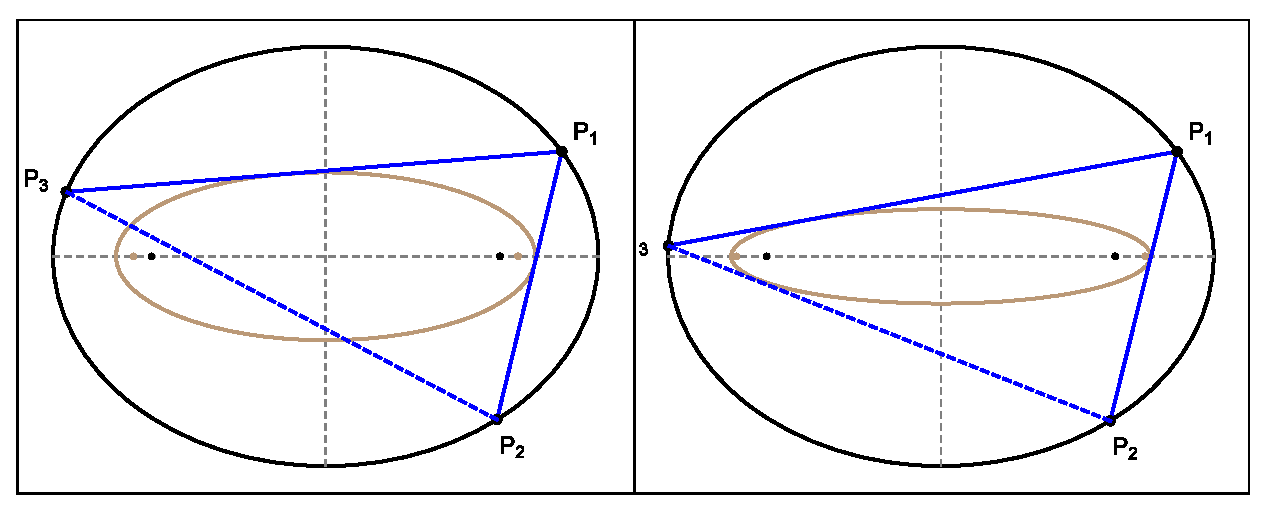
\includegraphics[width=\textwidth]{pics_03_070_ell_ints.eps}
    \caption{\textbf{Left:} Two concentric, axis-parallel ellipses (black and brown), and a point $P_1$ on the outer one. The lines thru $P_1$ tangent to the inner ellipse intersect the outer one at $P_2$ and $P_3$. Notice that $P_2 P_3$ cut thru the inner ellipse, i.e., the pair of ellipses does not satisfy Cayley's conditions. \textbf{Right:} the minor axis of the inner ellipse has been scaled such that $P_1 P_2 P_3$ is now a Poncelet triangle.}
    \label{fig:ell-ints}
\end{figure}

The intersection of these two lines with $\E$ are given by:

\begin{equation}\aligned
    P_2& =[\frac{A_{20} x_1 + A_{02} y_1}{b A_{11}} ,  \frac{B_{20} x_1 + B_{02} y_1}{a A_{11}} ]=[p_{2x},p_{2y}]\\
    P_3&=[\frac{A_{20} x_1 - A_{02} y_1}{b A_{11}},\frac{B_{20} x_1 - B_{02} y_1}{a A_{11}}=[p_{3x},p_{3y}]\\
    A_{20}&=b(a^4  b_c^4 -(a^2 -  a_c^2)^2 b^4  ) \\
    A_{02}&= 2 a ( (a^2 + a_c^2)b^2 - b_c^2a^2) \sqrt{ b^2  b_c^2 (a^2 -  a_c^2)  x_1^2 +  a_c^2 a^2 (b^2 -  b_c^2)  y_1^2 }\\
    A_{11}&=\frac{(a^2 (b^2 +  b_c^2) - a_c^2 b^2)^2 }{a^2 }x_1^2+ \frac{(a^2 (b^2 -  b_c^2) + a_c^2b^2)^2 }{b^2}y_1^2\\
    B_{20}&=2b( (b^2 +  b_c^2) a^2 -    a_c^2 b^2) \sqrt{ b^2  b_c^2 (a^2 -  a_c^2)  x_1^2 +  a_c^2 a^2(b^2 -  b_c^2)  y_1^2} \\
    B_{02}&= a(a_c^4b^4-a^4(b^2-b_c^2)^2)
     %=-a (a^2( b^2 -    b_c^2) -  a_c^2 %b^2) (a^2 (b^2 -   b_c^2) +  a_c^2 b^2)
    \label{eq:chap3_orb3}
\endaligned
\end{equation}

\subsection{Concentric, Axis-Parallel Pair}

\begin{figure}
    \centering
    \includegraphics[width=\textwidth]{pics_03_110_n3_affine.eps}
    \caption{\textbf{Left:} }
    \label{fig:n3-affine}
\end{figure}

\subsubsection{General Case}

\begin{itemize}
    \item Cayley's condition $a_c/a+b_c/b=1$
    \item Vertex Parametrization
    \[ \{ P_1,P_2,P_3\} \] given by \cref{eq:chap3_orb3}, with
     $a_c/a+b_c/b=1$.
    \item Figure
\end{itemize}

Below we introduce a few special cases.

\subsubsection{Confocal (aka. Elliptic Billiard)}
 \[ \{ P_1,P_2,P_3\} \] given by \cref{eq:chap3_orb3}, 
with
   \[ a_c=\frac{a(\delta-b^2)}{c^2}, \;\; b_c=\frac{b(a^2-\delta)}{c^2},\;\; \delta^2=a^4-a^2b^2+b^4, \; c^2=a^2-b^2\]
\subsubsection{with Incircle}
 \[ \{ P_1,P_2,P_3\} \] given by \cref{eq:chap3_orb3}, with $a_c=b_c=r=ab/(a+b)$.

\subsubsection{Billiard's Excentrals}
 \[ \{ P_1,P_2,P_3\} \] given by \cref{eq:chap3_orb3}, 
with the ellipse pair $\{ \E_e ,\E\}$, where
$
E_e$ is given by $x^2/a_e^2+y^2/b_e^2=1$, with
   \[ a_e=\frac{\delta+b^2}{a}, \;\; b_e=\frac{\delta+a^2)}{b}.  \]
\subsubsection{with Circumcircle}
 \[ \{ P_1,P_2,P_3\} \] given by \cref{eq:chap3_orb3}, with $a=b =R=a_c+b_c$.
\subsubsection{Homothetic}
 \[ \{ P_1,P_2,P_3\} \] given by \cref{eq:chap3_orb3}, with $a=2a_c,\; b=2b_c$.
 
\subsubsection{Dual}
%\textcolor{red}{Quem e o dual: é aquele cuja caustica é anti-homotetica a externa, ou seja $a'/b'=b/a$}
 \[ \{ P_1,P_2,P_3\} \] given by \cref{eq:chap3_orb3}, with $a_c=\lambda b,\; b_c=\lambda a$ and $\lambda= a b/(a^2+b^2)$.
 
\subsection{Non-Concentric, Axis-Parallel Pair}

\subsubsection{General Case}

\subsubsection*{Poristic (aka. Bicentric)}


\subsubsection*{Brocard's Porism}

\subsection{Concentric, Unaligned}

\subsection{Generic Pair}

A list of the elliptic loci of centers in the $X_{1}$ to $X_{200}$ range can be found \href{https://dan-reznik.github.io/why-so-many-ellipses/}{here}.